\documentclass[12pt]{beamer}
\usepackage[T1]{fontenc}
\usepackage{lmodern}
\usepackage[english]{babel}
\usetheme{Copenhagen}
\usepackage{listings}
\usepackage{xmpmulti}

\begin{document}
\author{Mats Hoem Olsen, Roy Granheim}
\title{Simulating animals}
\subtitle{The survivle of the lucky}
%\logo{}
\institute{Norwegian university of enviroment and biosciense}
\date{26/1-2021}
\subject{INF200}
%\setbeamercovered{transparent}
%\setbeamertemplate{navigation symbols}{}

\begin{frame}
\maketitle
\end{frame}

\section{Table of contents}
\begin{frame}
\tableofcontents
\end{frame}

\setcounter{section}{0}

\section{Animal logic}

\begin{frame}{general}
\begin{itemize}
\item<+-> feeding
\item<+-> breading % to be corrected when bothered
\item<+-> migrate
\item<+-> grow old
\item<+-> die
\end{itemize}
\pause This sounds like a song...
\end{frame}

\subsection{logic}

\begin{frame}{general}
\begin{block}{feeding}
Herbivore eat what they can, carnivore eat what's left.
\end{block}

\begin{block}{breeding}
\begin{enumerate}[<+->]
\item birth if fit
\item have enough fat
\item random
\end{enumerate}
\end{block}

\begin{block}{migasion}
\alt<2>{Move if it can.}{Mostely random...}
\end{block}
\end{frame}

\subsection{programming theory}

\begin{frame}{Theory}
\begin{enumerate}
\item type-casting to avoid pointer bugs
\item eval() to create general code.
\end{enumerate}
\end{frame}

\begin{frame}[fragile]

\begin{lstlisting}[language=Python,basicstyle=\small]
[n for n in dir(sys.modules["biosim.animal"]) 
if not re.match("(__)|(np)|(ran)|(animal)",n)]
\end{lstlisting}

\end{frame}

\section{Visuals}


\begin{frame}{Graphical information}
    \begin{wrapfigure}{r}{0.40\textwidth}
	\centering
    	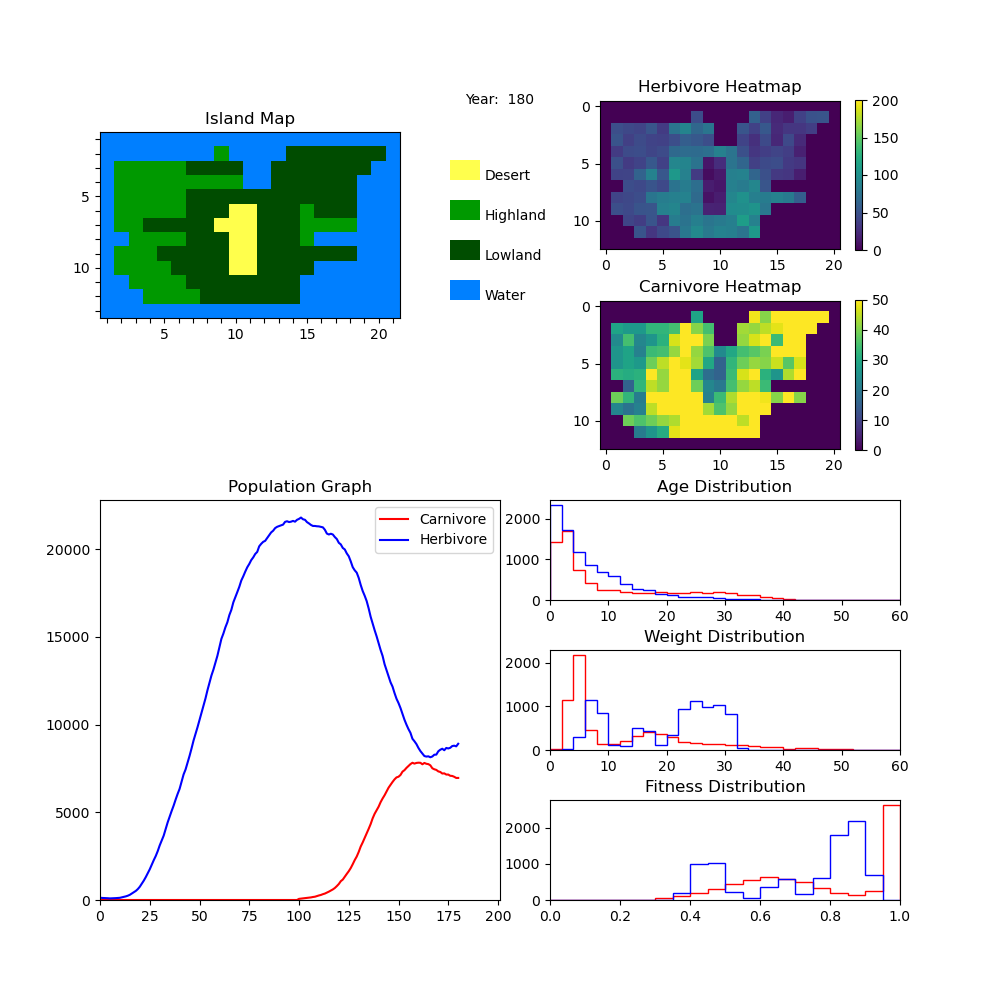
\includegraphics[scale=0.2]{test/test3_00180}
    \end{wrapfigure}
    Display features:
	\pause
    \begin{itemize}[<+->]
        \item Display current year
        \item Display the island geography
        \item Display informational graphs
        \item Ability to save images of the simulation
        \item Ability to set limits and graphical update step
    \end{itemize}
\end{frame}

\begin{frame}{Graphical handling}
    How does the graphics work?

    \pause 	1. The engine stores key information inside itself

    \pause 	2. The interface grabs that information

    \pause 	3. Then graphics takes information from the interface and processes it

\end{frame}


\begin{frame}{fin}
	\transduration<0-19>{0}
	\multiinclude[<+->][format=png, graphics={width=\textwidth}]{test/firework}
\end{frame}

\end{document}